%% ============================================================================
%% ADHD Assist — Paper 1 (ACM IUI 2027)
%% Overleaf: Compiler = pdfLaTeX · Main = main.tex
%% Layout: two-column ACM conference (sigconf).
%% For double-blind PCS submission, switch to:
%%   \documentclass[sigconf,anonymous,review]{acmart}
%% (the `anonymous` option is what printed "Anonymous Author(s)" / "Anon.")
%% ============================================================================
\documentclass[sigconf]{acmart}

\usepackage{booktabs}
\usepackage{graphicx}
\usepackage{xcolor}
\usepackage{balance}
\usepackage{tikz}
\usetikzlibrary{arrows.meta,positioning,fit,calc,shapes.geometric}

%% Quiet / clean ACM chrome for drafting
\setcopyright{none}
\settopmatter{printacmref=false}

\acmConference[IUI '27]{29th International Conference on
  Intelligent User Interfaces}{February 2027}{Helsinki, Finland}
\acmBooktitle{IUI '27: 29th International Conference on Intelligent User Interfaces,
  February 2027, Helsinki, Finland}
\acmYear{2027}
\copyrightyear{2027}
\acmDOI{XX.XXXX/XXXXXXX.XXXXXXX}
\acmISBN{978-1-4503-XXXX-X/27/02}

\author{Ahab Masud Siddiqui}
\affiliation{%
  \institution{University of British Columbia, Okanagan Campus}
  \city{Kelowna}
  \country{Canada}
}
\email{ahabmasudsiddiqui@gmail.com}

\author{Abdallah Mohamed}
\affiliation{%
  \institution{University of British Columbia, Okanagan Campus}
  \city{Kelowna}
  \country{Canada}
}
%% TODO: confirm supervisor's preferred contact email before submission
%% \email{...}

\renewcommand{\shortauthors}{Siddiqui and Mohamed}

\title[Enforcing ADHD-Supportive Structure in LLM Tutors]{%
  Beyond Prompting: Enforcing ADHD-Supportive Structure in LLM Tutors
  with a Second-Pass Oversight Layer}

\begin{abstract}
\input{sections/abstract}
\end{abstract}

\keywords{ADHD, accessibility, large language models, intelligent tutoring
systems, cognitive load, AI oversight, neurodivergence, user control}

\begin{CCSXML}
<ccs2012>
 <concept>
  <concept_id>10003120.10003121.10003129</concept_id>
  <concept_desc>Human-centered computing~Interactive systems and tools</concept_desc>
  <concept_significance>500</concept_significance>
 </concept>
 <concept>
  <concept_id>10003120.10003121.10003124.10010392</concept_id>
  <concept_desc>Human-centered computing~Accessibility systems and tools</concept_desc>
  <concept_significance>500</concept_significance>
 </concept>
 <concept>
  <concept_id>10010147.10010178.10010179</concept_id>
  <concept_desc>Computing methodologies~Natural language processing</concept_desc>
  <concept_significance>300</concept_significance>
 </concept>
</ccs2012>
\end{CCSXML}

\ccsdesc[500]{Human-centered computing~Interactive systems and tools}
\ccsdesc[500]{Human-centered computing~Accessibility systems and tools}
\ccsdesc[300]{Computing methodologies~Natural language processing}

%% General system diagram on page 1, directly under the title block.
\begin{teaserfigure}
\centering
%% Figure 1 — runtime control path (teaser width; uncrowded linear flow)
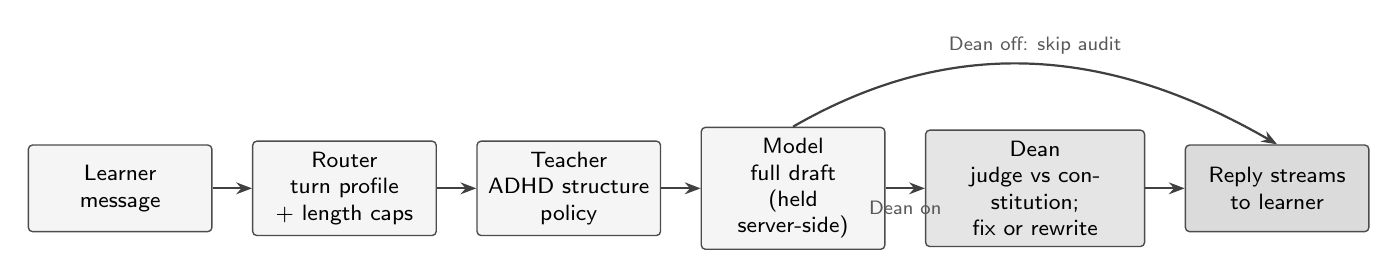
\begin{tikzpicture}[
  font=\sffamily\footnotesize,
  >=Stealth,
  node distance=5mm,
  stage/.style={
    draw=black!70, rounded corners=1.5pt, align=center,
    inner sep=4pt, minimum height=11mm, text width=20.5mm,
    fill=black!4, line width=0.5pt
  },
  dean/.style={stage, fill=black!10, text width=25mm},
  emit/.style={stage, fill=black!14},
  arr/.style={-{Stealth[length=2mm]}, thick, draw=black!75},
  lab/.style={font=\sffamily\scriptsize, text=black!65}
]
  \node[stage] (L) {Learner\\message};
  \node[stage, right=of L] (R) {Router\\turn profile\\+ length caps};
  \node[stage, right=of R] (T) {Teacher\\ADHD structure\\policy};
  \node[stage, right=of T] (M) {Model\\full draft\\(held server-side)};
  \node[dean, right=of M] (D) {Dean\\judge vs constitution;\\fix or rewrite};
  \node[emit, right=of D] (O) {Reply streams\\to learner};

  \draw[arr] (L) -- (R);
  \draw[arr] (R) -- (T);
  \draw[arr] (T) -- (M);
  \draw[arr] (M) -- node[lab, below, yshift=-1pt] {Dean on} (D);
  \draw[arr] (D) -- (O);
  \draw[arr] (M.north) to[out=30, in=150]
    node[lab, above, pos=0.5] {Dean off: skip audit} (O.north);
\end{tikzpicture}

\caption{ADHD Assist runtime path in EduAI. Router selects turn profile and
caps; Teacher applies structure policy; the model writes a full draft. If
Dean is on, the draft is audited against the constitution and may be fixed
before stream-out; if off, the draft emits unchecked. Adapted from Liu
et~al.'s Dean oversight cadence~\cite{liu2024socraticlm}.}
\Description{Flowchart from learner message through Router, Teacher policy,
model draft, optional Dean audit and rewrite, then stream to learner.}
\label{fig:pipeline}
\end{teaserfigure}

\begin{document}
\maketitle

\section{Introduction}
\label{sec:intro}

Students already treat LLM chat as an ordinary study tool. The product shows
up as a blank box and a stream of answers, which would pose no problem if
every answer were easy to scan and easy to re-enter after an interruption.

In practice it is not. Default replies look like essays: long continuous prose, several
threads in one answer, almost no help if you leave and come back. The design
assumes the reader can hold attention, keep the answer in working memory, and
pick up after a distraction. For many students with ADHD, those assumptions
are where accessibility breaks. Walls of text raise extraneous load. Missing
signposts make tab-switching expensive. Compound answers invite more drift on
the next turn.

So people try prompts. Students with ADHD (and instructors trying to help) ask
the model to ``summarize first,'' ``use three bullets,'' ``take one step at a
time,'' or ``don't digress.'' That can work for a turn. It rarely sticks for a
session. The model is trained to sound helpful and fluent; multi-turn context
pulls it back toward verbosity, topic-merge, and essay form. If ADHD support
only works when the user re-pleads for structure on every message,
accessibility depends on perfect prompting. That is not a reliable interactive
system.

The interface question, then, is larger than one better system prompt. What
should the tutoring product do when dialogue context drifts? We argue it has
to \emph{steer and check} generative replies, not just ask politely.

\paragraph{What this work does.}
Instead of accepting long, unstructured answers that can overwhelm students
with ADHD, we apply research-backed structure rules so tutoring replies stay
focused and clearly shaped. Then we verify each draft with a second AI before
the student sees it. Asking the model once to ``stay short'' is prompting.
Writing those rules into the system and checking every reply against them
before emit is \textbf{enforcement}. Making ADHD-supportive LLM tutoring
reliable is an enforcement problem, not a prompting problem.

That claim has consequences we can measure. Unconstrained models almost never
hold the scaffold we need. Putting the rules in the prompt recovers most of
it. A second-pass checker can add a further adherence gain without changing
the underlying model, retrieval, or tools. We also ran a small ADHD human
pilot (overload, comprehension, usability) as an early step toward inclusive
AI tutoring; we report it as a feasibility check rather than as confirmatory
proof that Assist reduces cognitive load.

We implement this approach inside \textbf{EduAI} as \textbf{ADHD Assist}.
Assist is a response-shape policy grounded in the literature (five pillars),
not a second chat product.

The enforcement piece is a Router$\to$Teacher$\to$Student$\to$\textbf{Dean}
pipeline adapted from Liu et~al.'s oversight
pattern~\cite{liu2024socraticlm}. The Dean's job is narrow. It judges a full
draft against a written constitution for structure (length, summary~/~Next?,
turn profile). When Assist+oversight is on, it may revise that draft
\emph{before} the learner sees it. Figure~\ref{fig:pipeline} shows the path
from learner message to stream-out.

One boundary matters up front. Guided Socratic discovery in a separate AiTutor
extension is related platform work. This paper's contribution is the
structural Assist layer in core chat. We do not claim that pedagogy here.

\subsection{Research questions}
\label{sec:rqs}

We keep four programme questions. They are not equal empirical claims in this
paper.

\begin{description}
  \item[RQ1] Which response attributes support ADHD learners?
    \emph{Role here:} design rationale (pillars + technique$\times$symptom
    mesh; mesh cells argued, not measured). Home: \S\ref{sec:design}.
  \item[RQ2] Can an LLM keep those patterns across multi-turn use?
    \emph{Role here:} supporting result (baseline drift vs assist arms).
    Home: \S\ref{sec:study1}.
  \item[RQ3] Does a second oversight layer improve adherence over prompting
    alone? \emph{Role here:} \textbf{primary research question.}
    Home: \S\ref{sec:system}--\ref{sec:study1}.
  \item[RQ4] Does Assist improve load~/~learning for ADHD students vs
    baseline? \emph{Role here:} protocol feasibility + descriptive human
    metrics only; \textbf{not} confirmatory. Home: \S\ref{sec:feasibility}.
\end{description}

\paragraph{Primary RQ (this paper).}
Does a second-pass oversight layer improve structural scaffold adherence over
prompting alone when multi-turn interaction causes drift?

\subsection{Contributions}

\begin{enumerate}
  \item \textbf{Design (\S\ref{sec:design}).}
    Five ADHD Assist pillars (concise, structured, progressively disclosed,
    single-focus, gentle redirect) and a theoretical technique $\times$
    symptom mesh that states which deficits each pillar is meant to repair,
    including honest under-coverage (reward~/~deep metacognition).
  \item \textbf{System (\S\ref{sec:system}).}
    An interactive control path in EduAI: same model, retrieval, tools, and
    temperature across arms; Assist = policy prepend $\pm$ Dean audit on a
    full draft before stream-out to the learner (style-only IV).
  \item \textbf{Measured ablation (\S\ref{sec:study1}).}
    On multi-turn probes (5$\times$ repeats, Gemini~2.5 Flash), baseline
    structural pass is \textbf{0\%}; assist-prompt-only reaches
    \textbf{67\%} strict~/~\textbf{76\%} turn-aware; assist+oversight reaches
    \textbf{71\%} strict~/~\textbf{80\%} turn-aware (late-turn turn-aware
    \textbf{86\%~$\rightarrow$~89\%}). The oversight lift is real but modest.
    Turn-aware pass is the primary metric for assist comparisons because
    strict scoring under-credits correct redirects.
\end{enumerate}

Alongside these contributions, a short within-person ADHD pilot (H26-00906;
$n{=}6$ analyzed) validated that the protocol and Assist toggle are operable
as a study task (\S\ref{sec:feasibility}). We report it as feasibility
validation only; powered human outcomes are left to a follow-on study.

The remainder of the paper reviews related work and the gap it leaves
(\S\ref{sec:related}), presents the design rationale (\S\ref{sec:design}) and
system (\S\ref{sec:system}), reports the synthetic evaluation
(\S\ref{sec:study1}) and the human feasibility pilot
(\S\ref{sec:feasibility}), and closes with discussion
(\S\ref{sec:discussion}) and limitations (\S\ref{sec:limitations}).

%% Renamed from "Background and Related Work" to the canonical A* section name.
\section{Related Work}
\label{sec:related}

Default LLM tutors reward fluent paragraphs. That design assumes the learner
can hold the whole turn in working memory, stay on one topic, and re-enter
after a tab switch. For many students with ADHD, those assumptions fail in
ordinary use. Prior work in three areas makes that failure predictable, yet
none of it closes the gap that ADHD Assist addresses.

\subsection{ADHD as a dimensional, multi-deficit condition}

Start with the condition itself: ADHD is not one ``attention off'' switch.
DSM-5 presentations (inattentive, hyperactive-impulsive, combined) sit on
severity ranges, and executive-function accounts go
deeper~\cite{apa2022dsm}. Barkley treats behavioral inhibition as core, with
secondary damage to working memory, internalized speech, affect and motivation
regulation, and reconstitution~\cite{barkley1997behavioral}. Brown clusters
activation, focus, effort, emotion, memory, and action~\cite{brown2013new}.
Adult evidence treats emotional dysregulation as more than a side
effect~\cite{beheshti2020emotion}. Sonuga-Barke's dual pathway adds delay
aversion and reward-motivation alongside executive
dysfunction~\cite{sonuga2003dual}, so interest and near-term payoff can mask
or amplify the same deficits.

\paragraph{What we take.}
Tutoring has to name \emph{which} deficit a reply shape is meant to repair
(working memory, initiation, impulsivity, set-shifting, affect), not only
``make chat nicer.''
\paragraph{What we cannot claim from taxonomy alone.}
That any particular UI or prompt \emph{works} until it is measured under use.

The closest GenAI bridge is Zhu, Yu, and Luo~\cite{zhu2026scaffolding}. ADHD
university students and experts co-design scaffolding that limits the visible
agenda, prefers progressive tasks, and warns against cognition outsourcing and
clinical overclaim. We take their interaction directions as primary
human-grounded inspiration for the pillars. We do not treat their study as a
measured evaluation of EduAI.

\subsection{Cognitive load and accessibility foundations}

Even if the diagnosis is clear, packaging still matters. Cognitive load theory
separates intrinsic task demand from extraneous packaging and germane
work~\cite{sweller2011cognitive}. Extraneous load rises when answers dump
undifferentiated text. Working memory typically holds only a few chunks at
once~\cite{cowan2010magical}. Accessibility guidance makes that concrete:
W3C~COGA pushes clear purpose, hierarchy, plain language, and predictable
structure, and names AD(H)D among populations that
benefit~\cite{w3c2021coga}. Mayer's segmenting, signaling, and coherence
principles~\cite{mayer2021multimedia}, and UDL's multiple means of
representation~\cite{cast2018udl}, point the same way: signpost, chunk, and do
not overwhelm the first surface.

\paragraph{What we take.}
Length caps, summary-first layout, and one-decision-at-a-time disclosure are
load-management techniques with established warrants. They are not decorative
``AI style.''
\paragraph{What we cannot claim.}
That CLT or COGA alone prove ADHD-specific superiority over neurotypical
learners. Those frameworks are general. Whether Assist helps students with
ADHD \emph{more} than peers is powered human follow-on work, not this paper's
primary result.

\subsection{LLM tutoring architecture and enforcement}

A third literature designs LLM tutors as \emph{pipelines}, not single prompts.

Liu et~al., SocraticLM, introduce a Dean--Teacher--Student pattern: a Dean
judges whether a generated turn meets stated requirements and may revise it
before presentation to the learner~\cite{liu2024socraticlm}. They also score
tutor readability, productive refusal of irrelevant moves, and
validate-and-move. We take the oversight \emph{cadence} and the
readability~/~redirect vocabulary. We do \textbf{not} claim their Socratic
fine-tuning gains or those score numbers as ours. Those metrics stay parked
for later EduAI instrumentation.

Saha, Hase, and Bansal show selective explanation can beat always-explain,
that style exemplars beat long rule lists for compliance, and that a
\emph{misaligned} teacher harms the trajectory~\cite{saha2023can}. This is
perhaps the strongest evidence that prompting alone is fragile. Shani et~al.\ treat a
written \emph{constitution} of tutoring quality over full dialogues and treat
multi-topic teacher turns as violations~\cite{shani2024multiturn}; our
single-focus pillar and Dean constitution borrow that framing. Chevalier
et~al.\ warn that dialogue or style tuning without content checks can break
subject accuracy~\cite{chevalier2024lmscience}, so oversight here must aim at
\textbf{structure}, not inventing facts (key-point style grading motivates our
content-parity discipline). Choudhury and Sodhi (\emph{Better than your
teacher}~/~LEAP) argue for privileged teachers that see full drafts before a
weak agent acts~\cite{choudhury2025better}; we take the
full-draft-before-stream idea only as architectural analogy. Their benchmarks
are not tutoring.

Ma et~al.\ support simulated-learner QA infrastructure~\cite{ma2025students}.
Big Five is not ADHD, so that line is useful for harnesses, not clinical
claims. Heterogeneous-learner teaching theory (e.g., Zhang et~al.\
MINT~\cite{zhang2023nonparametric}) motivates personalisation only at a high
level. It does not justify a user-facing ADHD rule by itself.

\subsection{Gap}
\label{sec:gap}

The components needed for a solution already exist in prior work. Zhu et~al.\
show what ADHD-friendly scaffolding looks like in design workshops. Sweller,
Cowan, and the W3C~COGA guidance explain why short, hierarchical, predictable
replies reduce extraneous load. Saha et~al.\ and Shani et~al.\ show that
teaching style needs selective policy and a written constitution, because
open prompting is fragile. Liu et~al.\ (and LEAP-style full-draft review)
show that a second agent can judge a turn and revise it before the learner
sees it.

What is missing is a single working tutoring control path that combines them.
Two connections are required, and no prior system provides both. The first is
design clarity: assembling the already-known technique-to-deficit warrants
(from ADHD research, load theory, and co-design) into one explicit technique
$\times$ deficit mesh for a tutoring product, and treating that mesh as the
design constitution (\S\ref{sec:design}). The mapping is literature-grounded;
Study~1 does not re-prove every cell as a clinical outcome. The second is
system evaluation: writing that mesh as a runtime policy, adding a verifying
second agent, and measuring structural adherence under multi-turn drift in
three arms (baseline, prompt-only, oversight) while holding model, retrieval,
and tools fixed. That is the appropriate test of whether enforcement beats
prompting when dialogue context pulls the tutor off-scaffold.

The closest prior systems stop one step short. Zhu et~al.\ motivate the
patterns, but they do not run an enforceable Dean on a live tutor under drift
probes. SocraticLM does include a Dean, yet its constitution is Socratic
pedagogy, not ADHD load~/~structure rules, and it does not report our
prompt-vs-oversight ablation. Selective-teaching and RLHF-education papers
motivate policy and audit in general; they do not target ADHD scaffolds or
late-turn structural pass under interruptions.

This paper addresses that gap. We design the mesh, instantiate a
Router / Teacher / Student / Dean control path in EduAI as
control over reply shape, and measure whether oversight beats prompting under
multi-turn drift. Human load and learning stay feasibility-only until we have
powered evidence.

\section{Design Rationale: ADHD Assist Pillars}
\label{sec:design}

\begin{table*}[t!]
\caption{Technique $\times$ symptom mesh for ADHD Assist. Cells are design
ratings from prior evidence and our synthesis, not Study~1 clinical outcomes.
Columns: Sust.\ = sustained attention; WM = working memory; Init.\ = task
initiation; Imp.\ = impulsivity; Infl.\ = inflexibility; Rew.\ =
reward~/~motivation; Emot.\ = emotional dysregulation; Meta.\ = metacognition.}
\label{tab:mesh}
\centering
\footnotesize
\setlength{\tabcolsep}{4.5pt}
\begin{tabular}{l*{9}{c}}
\toprule
Technique & Sust. & WM & Init. & Imp. & Time & Infl. & Rew. & Emot. & Meta. \\
\midrule
P1 Concise & \textbf{S} & \textbf{S} & \textbf{S} & I & P & I & P & I & n \\
P2 Structured & \textbf{S} & \textbf{S} & \textbf{S} & P & P & P & I & I & P \\
P3 Progressive & \textbf{S} & \textbf{S} & \textbf{S} & P & P & I & P & I & P \\
P4 Single-focus & \textbf{S} & P & P & \textbf{S} & I & \textbf{S} & I & I & P \\
P5 Gentle redirect & \textbf{S} & I & n & \textbf{S} & P & \textbf{S} & I & \textbf{S} & P \\
\bottomrule
\end{tabular}
\end{table*}

If default LLM tutoring fails students with ADHD, what should a reply look
like instead?

ADHD Assist uses five \textbf{response-shape} pillars. They draw on cognitive
load and accessibility research~\cite{sweller2011cognitive,cowan2010magical,w3c2021coga},
ADHD executive-function accounts~\cite{barkley1997behavioral}, and ADHD
co-design evidence from Zhu, Yu, and Luo~\cite{zhu2026scaffolding}. We mapped
each technique to the ADHD difficulties it is meant to help. The pillars
become the Teacher policy and the Dean's written constitution
(\S\ref{sec:system}).

Study~1 tests whether the structural signature of these pillars holds under
multi-turn use when a Dean is present; it does not re-test every symptom
claim as a clinical outcome. The mesh ratings in this section
(Strong~/~Partial~/~Indirect) are likewise design ratings from the literature
and our synthesis.

\subsection{The five pillars}
\label{sec:pillars}

\paragraph{P1. Concise.}
Working memory only holds a few chunks at once~\cite{cowan2010magical}. Long
undifferentiated text raises extraneous load~\cite{sweller2011cognitive} and
is hard to re-enter after an interruption~\cite{zhu2026scaffolding}.

\emph{In practice:} tutoring aims about 150 words (hard cap 250); clarifications
shorter. No filler praise. If the topic exceeds the cap, summarize and invite
continuation (P3).

\emph{When it fails:} lectures, repeated reassurance, answer buried under
throat-clearing.

\paragraph{P2. Structured.}
Headings, bullets, and a fixed order externalize ``where am I?'' so the
learner does not rebuild context from prose after
interruption~\cite{w3c2021coga,barkley1997behavioral}. SocraticLM scores tutor
readability for the same reason~\cite{liu2024socraticlm}.

\emph{In practice:} scaffolded turns open with a short summary block and close
with one continuation invite; optional step ladder (at most five) and at most
one quick check. Scoring anchors are Top summary and Next?. The interface may
label those blocks TLDR and Continue; the underlying checks are unchanged.

\emph{When it fails:} free-form essay; missing summary or Next?; nested
sprawl.

\paragraph{P3. Progressively disclosed.}
One decision surface at a time beats dumping everything up
front~\cite{saha2023can,zhu2026scaffolding}.

\emph{In practice:} answer the immediate ask tightly first. Add depth only
after an explicit Next? invite. If the user asks two questions, answer the
first and defer the second.

\emph{When it fails:} full plan or lecture in one shot; multiple open threads.

\paragraph{P4. Single-focus.}
Multiple agendas leave attention residue and invite topic-merge when
inhibition is weak~\cite{sweller2011cognitive,zhu2026scaffolding,shani2024multiturn}.

\emph{In practice:} one main topic per turn. Steps serve that topic only.

\emph{When it fails:} two unrelated headings; silently answering a second
injected topic.

\emph{Limit:} policy and redirect handling encode this intent. Automatic
topic-count detection is weak, so Study~1 uses scripted interrupt probes
rather than relying on an automatic one-topic detector.

\paragraph{P5. On-task continuity (gentle redirect).}
Off-topic jumps are common for many students with ADHD. Harsh refusal raises
frustration~\cite{beheshti2020emotion,zhu2026scaffolding}. SocraticLM scores
productive handling of irrelevant moves~\cite{liu2024socraticlm}.

\emph{In practice:} acknowledge the jump, name the prior topic briefly, offer
return or switch, without scolding.

\emph{When it fails:} silent tangent-follow, or a blunt ``I can't help with
that.''

\subsection{Supporting constraints (not separate IVs)}

Still enforced, but not the main style attributes under test:
\begin{itemize}
  \item \textbf{Validate and move:} confirm a correct grasp, then advance
    (SocraticLM validate-and-move analogue~\cite{liu2024socraticlm}).
  \item \textbf{Honest unknowns:} do not invent course facts.
  \item \textbf{No clinical inference} from chat.
  \item \textbf{Learner-owned reflection:} optional; off in Study~1 so style
    remains the only planned difference.
\end{itemize}

The Dean (\S\ref{sec:system}) audits the pillars through a written
constitution. It is not a sixth pillar.


\subsection{Technique $\times$ symptom mesh}
\label{sec:mesh}

Prior ADHD, load, and co-design work already links reply techniques to
specific difficulties: short chunked answers to working-memory
limits~\cite{cowan2010magical,sweller2011cognitive}; external structure to
re-entry and attention~\cite{barkley1997behavioral,w3c2021coga}; progressive
disclosure to initiation and overload~\cite{saha2023can,zhu2026scaffolding};
single-focus to impulsivity and topic-merge~\cite{shani2024multiturn}; gentle
redirect to disruption and emotional
dysregulation~\cite{zhu2026scaffolding,beheshti2020emotion,liu2024socraticlm}.

We assemble those links into one technique $\times$ deficit mesh for ADHD
Assist and rate each cell from that evidence. Table~\ref{tab:mesh} is the
design map (\textbf{S}~=~strong intended help; \textbf{P}~=~partial;
\textbf{I}~=~indirect; \textbf{n}~=~not claimed). Systems that ship structure
or a second-pass checker usually motivate the technique; they less often
publish this matrix as an explicit product constitution.

P1--P3 carry the working-memory, attention, and initiation core. P4--P5 carry
impulsivity and set-shifting when the session derails. Emotional dysregulation
is addressed mainly by redirect tone (P5), not a separate affect model.
Reward~/~motivation and deep metacognition are weakly covered here; richer
engagement pedagogy sits outside this paper's independent variable.

\subsection{Hand-off to system and Study~1}

Pillars become Teacher policy. The constitution becomes the Dean checklist.
Turn profiles decide when the full scaffold applies versus a redirect.
Study~1 tests whether that structural signature sticks better with a Dean
than with prompting alone.

\section{System: Instantiation in EduAI}
\label{sec:system}

\begin{figure*}[t]
\centering
%% Figure 2 — three Study 1 arms (compact; fits figure* width)
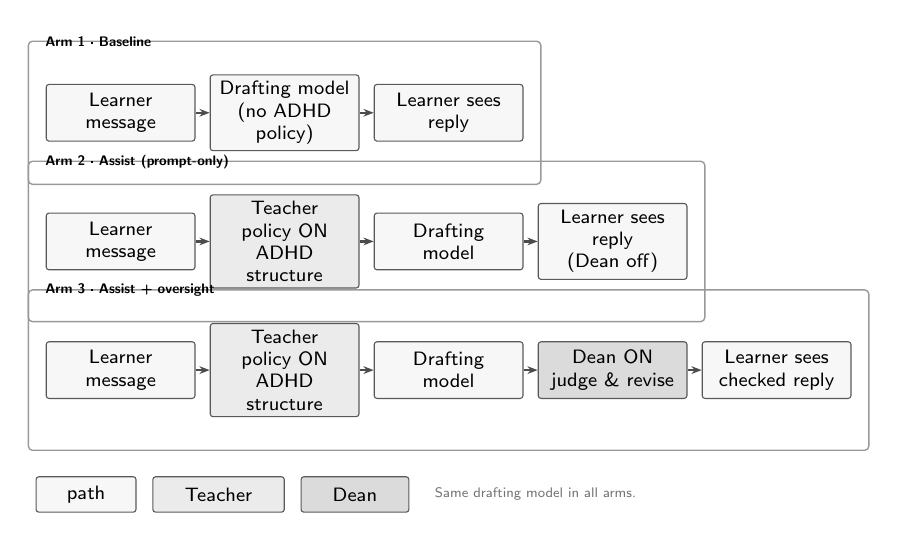
\begin{tikzpicture}[
  font=\sffamily\scriptsize,
  >=Stealth,
  node distance=1.6mm and 1.8mm,
  box/.style={
    draw=black!65, rounded corners=1pt, align=center,
    inner sep=2.4pt, minimum height=7.2mm, text width=17.2mm,
    fill=black!3, line width=0.4pt
  },
  policy/.style={box, fill=black!8},
  dean/.style={box, fill=black!14},
  arr/.style={-{Stealth[length=1.3mm]}, thick, draw=black!70},
  arm/.style={
    draw=black!40, rounded corners=1.5pt, inner sep=2.8pt,
    line width=0.5pt
  },
  title/.style={font=\sffamily\tiny\bfseries, anchor=west}
]
  %% Arm 1
  \node[box] (b1) {Learner\\message};
  \node[box, right=of b1] (b2) {Drafting model\\(no ADHD policy)};
  \node[box, right=of b2] (b3) {Learner sees\\reply};
  \draw[arr] (b1) -- (b2);
  \draw[arr] (b2) -- (b3);
  \node[arm, fit=(b1)(b2)(b3), inner ysep=4.2mm, inner xsep=2.2mm] (B) {};
  \node[title] at ([xshift=1mm,yshift=-0.15mm]B.north west) {Arm 1 · Baseline};

  %% Arm 2
  \node[box, below=9mm of b1] (p1) {Learner\\message};
  \node[policy, right=of p1] (p2) {Teacher policy ON\\ADHD structure};
  \node[box, right=of p2] (p3) {Drafting\\model};
  \node[box, right=of p3] (p4) {Learner sees\\reply (Dean off)};
  \draw[arr] (p1) -- (p2);
  \draw[arr] (p2) -- (p3);
  \draw[arr] (p3) -- (p4);
  \node[arm, fit=(p1)(p2)(p3)(p4), inner ysep=4.2mm, inner xsep=2.2mm] (P) {};
  \node[title] at ([xshift=1mm,yshift=-0.15mm]P.north west) {Arm 2 · Assist (prompt-only)};

  %% Arm 3
  \node[box, below=9mm of p1] (o1) {Learner\\message};
  \node[policy, right=of o1] (o2) {Teacher policy ON\\ADHD structure};
  \node[box, right=of o2] (o3) {Drafting\\model};
  \node[dean, right=of o3] (o4) {Dean ON\\judge \& revise};
  \node[box, right=of o4] (o5) {Learner sees\\checked reply};
  \draw[arr] (o1) -- (o2);
  \draw[arr] (o2) -- (o3);
  \draw[arr] (o3) -- (o4);
  \draw[arr] (o4) -- (o5);
  \node[arm, fit=(o1)(o2)(o3)(o4)(o5), inner ysep=4.2mm, inner xsep=2.2mm] (O) {};
  \node[title] at ([xshift=1mm,yshift=-0.15mm]O.north west) {Arm 3 · Assist + oversight};

  %% legend
  \node[box, minimum height=4.5mm, text width=11mm, below=3.2mm of O.south west, anchor=north west, xshift=1mm] (lg1) {path};
  \node[policy, minimum height=4.5mm, text width=15mm, right=2mm of lg1] (lg2) {Teacher};
  \node[dean, minimum height=4.5mm, text width=12mm, right=2mm of lg2] (lg3) {Dean};
  \node[font=\sffamily\tiny, text=black!55, right=2mm of lg3] {Same drafting model in all arms.};
\end{tikzpicture}

\caption{Three Study~1 arms on the Teacher--Dean control stack.
Baseline uses the drafting model alone. Prompt-only Assist adds the ADHD
structure policy but skips Dean. Oversight adds Dean judge-and-revise before
the learner sees the reply. Same drafting model in all arms.}
\Description{Three horizontal pipelines comparing baseline, prompt-only
Assist, and Assist with Dean oversight.}
\label{fig:threearms}
\end{figure*}

ADHD Assist is not a second chat product. It is a mode inside EduAI chat: a
toggle, a structure policy, and an optional second-pass check before the
learner sees the reply.

When the mode is off, EduAI tutors as usual. When it is on, the model,
retrieval, tools, and temperature stay the same. What changes is whether
replies are asked to follow an ADHD-supportive shape, and whether that shape
is checked before emit.

\subsection{The Dean-guided pipeline}
\label{sec:pipeline}

Liu et~al.\ use a \textbf{Dean--Teacher--Student} pipeline for tutoring
dialogues~\cite{liu2024socraticlm}. Three LLM agents interact. The Dean judges
whether the Teacher's turn meets stated teaching requirements and may revise
that turn before the Student sees it. That judge-and-revise step is the piece
we keep.

We adapt the pattern for ADHD Assist in EduAI. Two differences matter:
\begin{enumerate}
  \item Our final audience is a \textbf{human learner}, not a simulated
    Student agent.
  \item We add a \textbf{Router} that decides turn type before generation.
    SocraticLM does not have that gate.
\end{enumerate}

Study~1 then turns the adapted stack into three enforcement depths.
Figure~\ref{fig:threearms} is that comparison (Figure~\ref{fig:pipeline} in
\S\ref{sec:intro} is the single runtime flowchart with Router detail).


\paragraph{Router.}
The Router runs first on Assist-on turns. It assigns a turn profile (full
tutoring, brief clarification, redirect, greeting, confirmation, meta). That
profile decides whether the full scaffold is required and whether the Dean may
intervene. Without it, Assist would hang a tutoring template on everyday
``thanks'' messages. Baseline skips Assist, so it also skips this
Assist-scoped routing.

\paragraph{Teacher.}
When Assist is on, the ADHD Assist policy is prepended to the system prompt
(scoped by profile). Those rules are the requirements the Dean later checks.
In Study~1, the \textbf{prompt-only} arm stops here: Teacher on, Dean off.

\paragraph{Drafting model.}
EduAI's ordinary generation path writes the first-pass reply in every arm.
When oversight is on, the draft is held server-side so the Dean sees a
complete answer, not a half-streamed fragment. The learner does not read the
raw first pass when the Dean is scheduled to run.

\paragraph{Dean.}
The Dean is the oversight role. It judges whether the draft meets the ADHD
Assist constitution for this profile. If not, it revises before presentation:
deterministic structural fixes when possible, otherwise a second model
rewrite. Greeting, confirmation, and meta turns skip the Dean. We supervise
\textbf{structure}, not Socratic questioning style. In the runs reported
here, the Dean is served by the same model as the drafting model
(\texttt{google:gemini-2.5-flash}). Running the Dean on a separately sized
model is possible in the architecture but is not evaluated in this paper;
exploratory capacity notes and a quality--latency--cost follow-on appear in
Section~\ref{sec:limitations}. The Dean appears only in the oversight arm of
Figure~\ref{fig:threearms}.
Table~\ref{tab:arms} summarizes what is on in each arm.

\begin{table}[t]
\caption{Study~1 arms: what is on for each enforcement depth.}
\label{tab:arms}
\small
\centering
\begin{tabular}{@{}lll@{}}
\toprule
Arm & Teacher policy & Dean \\
\midrule
Baseline & off & off \\
Prompt-only & on & off \\
Oversight & on & on \\
\bottomrule
\end{tabular}
\end{table}

\subsection{Style is the only planned difference}
\label{sec:iv}

Across Study~1 arms we freeze the chat model, retrieval, tools, temperature,
and streaming contract. We only change whether the Teacher policy is prepended
and whether the Dean runs. Second-pass latency is an engineering cost of
oversight, not a second research factor; we have not systematically measured
latency distributions and report no latency outcomes here.

This paper claims the ADHD Assist structural layer in EduAI core chat. Guided
discovery on a separate tutoring surface is related platform work, not this
contribution.

\subsection{Turn profiles}
\label{sec:profiles}

Table~\ref{tab:profiles} lists when the full scaffold and the Dean apply.

\begin{table}[b]
\caption{Turn profiles: when full scaffold and Dean apply.}
\label{tab:profiles}
\small
\centering
\begin{tabular}{@{}lll@{}}
\toprule
Profile & Full scaffold? & Dean? \\
\midrule
Full tutoring, brief clarification & yes & yes, if draft fails \\
Redirect & no (boundary template) & yes, if template fails \\
Greeting, confirmation, meta & no & no \\
\bottomrule
\end{tabular}
\end{table}

Study~1 therefore reports \textbf{turn-aware (profile) pass} as the primary
comparison between assist arms: a correct redirect should not be forced into
a Top summary block. The interface may show TLDR~/~Continue; metrics still
use Top summary~/~Next?.

\subsection{What the Dean may change}

The constitution asks three questions:
\begin{enumerate}
  \item Does the draft match the shape required for this profile?
  \item Is it under the word cap and single-focus rules when those apply?
  \item Can we restore compliance without inventing course facts?
\end{enumerate}

The Dean may restore markers, trim over-cap text, and push redirects onto the
boundary template. It is not a second tutor rewriting pedagogy. Until a
sampled content-parity audit is published, Results claim scaffold adherence
only, not that structure changes never touch facts.

\subsection{Hand-off to Study~1}

Study~1 runs the same synthetic turns through the same system and model at
three enforcement depths (baseline, prompt-only, oversight), which is exactly
the contrast the primary research question requires.

\section{Study 1: Methods and Results}
\label{sec:study1}

\subsection{What we manipulate}

We ask one primary question. When a tutoring scaffold starts to fall apart
over multiple turns, does a second-pass oversight step hold the structure
better than putting the same rules in the prompt alone?

To answer that, we only change how ADHD-supportive structure is enforced.
Everything else stays fixed: the same chat model
(\texttt{google:gemini-2.5-flash} for the reported runs), the same retrieval,
tools, and temperature, and the same synthetic user turns.

That gives three arms (Figure~\ref{fig:threearms}):
\begin{enumerate}
  \item \textbf{Baseline:} ordinary tutoring; Assist off.
  \item \textbf{Assist, prompt-only:} ADHD Assist policy in the teacher system
    prompt; no second pass.
  \item \textbf{Assist + oversight:} same policy, plus a Dean that reads the
    full draft and revises when the constitution fails.
\end{enumerate}

The independent variable is not a smarter model or better retrieval. It is
whether structure is requested in the prompt, or checked after generation.

\subsection{What we measure}

We score each assistant turn for structural adherence with an automatic
checker.

\paragraph{Strict checklist.}
The reply must include a summary-first marker, end with a continue invite, and
stay under the word cap. Harsh on short redirects that correctly refuse a full
teaching template.

\paragraph{Turn-aware checklist (primary for Assist comparisons).}
Same idea, but a redirect may use the short boundary template instead of the
full tutoring scaffold. That is the fairer primary score when comparing
prompt-only to oversight.

\paragraph{Interface labels.}
The live UI may show TLDR and Continue where the system stores and scores Top
summary and Next?. Study~1 scores the internal anchors.

We also keep a late-turn aggregate (second-and-later turns in a scenario, and
the late tranche of the long probe), because that is where prompt drift shows
up if it is going to. The headline result is the automated pass rates on the
three-arm freeze.

\subsection{Probes}

All Study~1 inputs are synthetic multi-turn tutoring scenarios. No learner
accounts. No personal data. We average five independent repeats per arm. The
freeze includes a multi-turn topic interruption (core drift), continue-a-plan
after a break (re-orientation), and shorter and longer variants in the same
suite so we do not overfit to two scripts.

\subsection{How we ran the freeze}

Each arm ran as its own server configuration (oversight is a process-level
flag). We stored run metadata (git SHA, model id, arm label) with turn-level
results. For each arm we report the mean pass rate across five repeats, with
the observed range. These are measured compliance rates under a fixed harness,
not population estimates with confidence intervals.

\subsection{What Study 1 deliberately is not}

Study~1 does not measure cognitive load, learning gain, or preference; those
belong to the human protocol (\S\ref{sec:feasibility}). Study~1 asks whether
the scaffold stays on the page when we ask the system to keep it there.

\subsection{Results}
\label{sec:study1results}

Table~\ref{tab:freeze} reports mean structural pass rates over five repeats on
the frozen multi-turn suite (\texttt{google:gemini-2.5-flash}).

\begin{table}[t]
\caption{Structural adherence on the multi-turn probe suite (mean; ranges in
parentheses). Turn-aware scoring allows correct redirects to use a short
boundary template; strict scoring demands full tutoring markers on every
turn.}
\label{tab:freeze}
\footnotesize
\centering
\setlength{\tabcolsep}{4pt}
\begin{tabular}{lccc}
\toprule
Metric & Baseline & Prompt-only & Oversight \\
\midrule
Overall (turn-aware)
  & 0\% (0--0\%)
  & \textbf{76\%} (50--93\%)
  & \textbf{80\%} (71--86\%) \\
Late-turn (turn-aware)
  & 0\% (0--0\%)
  & \textbf{86\%} (71--100\%)
  & \textbf{89\%} (86--100\%) \\
Overall (strict)
  & 0\% (0--0\%)
  & 67\% (50--79\%)
  & 71\% (64--79\%) \\
Late-turn (strict)
  & 0\% (0--0\%)
  & 77\% (71--86\%)
  & 80\% (71--86\%) \\
\bottomrule
\end{tabular}
\end{table}

Baseline is \textbf{0\% (0--0\%)} on both checklists across five repeats:
unconstrained replies still answer the probes, but they never emit the
required ADHD-supportive shape. That zero is not a straw man: it is what the
deployed default tutor produces under the same probes, so the informative
contrast for this paper is prompt-only vs oversight. Prompt-only Assist
produces the large jump
(turn-aware \textbf{76\%} overall~/~\textbf{86\%} late; strict \textbf{67\%}~/
\textbf{77\%}). Oversight adds a further lift (turn-aware \textbf{80\%}~/
\textbf{89\%} late; strict \textbf{71\%}~/~\textbf{80\%}), about four points
in aggregate, with larger gains on residual hard turns (plan resume and
post-interrupt failures that the prompt arm still misses). Strict
rates run lower than turn-aware because intentional redirects fail a
full-marker checklist by design; we claim scaffold adherence here, not content
invariance under Dean rewrite.

\section{Human Feasibility Pilot}
\label{sec:feasibility}

This paper's primary evidence is Study~1. We additionally ran a small
within-person ADHD pilot under ethics approval \textbf{H26-00906} to check
that Assist could be administered as a study task. Each participant used the
tutor twice (Assist off vs Assist on with second-pass oversight; order
counterbalanced) and completed NASA-TLX~\cite{hart1988nasa},
SUS~\cite{brooke1996sus}, brief UX items, a main-ideas comprehension item, and
preference questions after each mode.

Of nine Qualtrics records, seven were finished and \textbf{$n{=}6$} entered
paired means. All six analyzed responses were ADHD self-identified and were
collected while the instrument was still on Qualtrics preview links rather than
the final anonymous survey link, so we treat them strictly as pilot data for
validating the protocol, not as confirmatory study outcomes. One finished
response was excluded because categorical Assist preference contradicted that
participant's own SUS and TLX change (SUS fell and raw workload rose under
Assist despite an Assist preference), which we treat as a response-order or
technical confound.

\begin{table}[t]
\caption{Paired descriptives for the ADHD feasibility pilot ($n{=}6$;
preview distribution). Means (SD); $\Delta$ is Assist$-$Baseline.
Paired $|d|$ uses $\mathrm{mean}(\mathrm{Baseline}-\mathrm{Assist})/
\mathrm{SD}(\mathrm{Baseline}-\mathrm{Assist})$; for load metrics a positive
$d$ favors Assist, for benefit metrics we report absolute $|d|$ with the
Assist-favoring direction noted. With $n{<}30$, treat as descriptive only.}
\label{tab:pilot}
\small
\centering
\setlength{\tabcolsep}{3.5pt}
\begin{tabular}{lcccc}
\toprule
Metric & Baseline & Assist & $\Delta$ & $|d|$ \\
\midrule
TLX raw workload $\downarrow$
  & 3.71 (1.51) & 2.21 (0.99) & $-1.50$ & 0.94 \\
Cognitive load index $\downarrow$
  & 3.92 (1.83) & 2.08 (0.86) & $-1.83$ & 0.98 \\
SUS (0--100) $\uparrow$
  & 58.89 (21.82) & 80.28 (16.75) & $+21.39$ & 0.84 \\
Comprehension (main ideas) $\uparrow$
  & 3.67 (1.21) & 5.83 (1.17) & $+2.17$ & 1.06 \\
Felt oriented in app $\uparrow$
  & 4.00 (1.79) & 5.33 (1.03) & $+1.33$ & 1.29 \\
Layout easy to scan $\uparrow$
  & 4.33 (2.34) & 5.83 (0.98) & $+1.50$ & 0.55 \\
\bottomrule
\end{tabular}
\end{table}

Table~\ref{tab:pilot} reports the paired descriptives. Within this
feasibility cell, every listed mean moves Assist-ward: lower TLX raw workload
and cognitive-load index, higher SUS, comprehension, scan, and orientation
ratings, with large paired $|d|$ on several composites. Overall preference
favored Assist for $5/6$ participants (none preferred Baseline; one reported
no preference). The protocol and Assist toggle are operable as a study task.
These numbers do \textbf{not} confirm reduced load or ADHD-specific benefit in
the population. Powered human efficacy through the final distribution pipeline,
and any ADHD vs non-ADHD interaction, remain follow-on work.

\section{Discussion}
\label{sec:discussion}

The primary question is narrow: when multi-turn tutoring causes
ADHD-supportive scaffolds to slip, does second-pass oversight improve
structural adherence over a structure policy in the prompt alone?

Study~1 gives a three-part answer. Unconstrained tutoring almost never produces
the required scaffolds (\textbf{0\%}). The ADHD Assist policy recovers most of
the structure ($\sim$\textbf{76\%} turn-aware overall; $\sim$\textbf{86\%}
late). Oversight adds a further, measured but modest lift
($\sim$\textbf{80\%}~/~$\sim$\textbf{89\%} late), with larger gains on residual
hard turns. The aggregate gain from oversight is modest; the more important
contribution is architectural.

The takeaway is not that oversight replaces prompting. Reliable
ADHD-supportive structure is a \textbf{control stack}: written policy,
turn-aware routing, and an optional auditor that can revise a draft before the
learner sees it. Prompting does most of the work. Oversight is residual
insurance for multi-turn failure modes the prompt does not fully close. For a
tutor that must keep ADHD-supportive structure on by default, that stack is
the contribution: steering generative replies at the interface, with model,
retrieval, tools, and decoding held fixed.

We measured scaffold presence under automated checks. Hallucination motivated
the desire for control but was not a primary dependent variable. The human
pilot ($n{=}6$; Table~\ref{tab:pilot}) shows the protocol is operable and
paired descriptives lean Assist-ward; that is feasibility evidence, not a
population claim. Whether Assist helps students with ADHD \emph{more} than
their peers is a question for the powered follow-on study.

The modest oversight lift still supports the enforcement thesis, provided the
claim is kept at its actual size. We do not claim near-perfect overall rates,
confirmatory load reduction, or ADHD exclusivity.

Model capacity is a separate follow-on question. Study~1 freezes one drafting
model and uses that same model for Dean rewrites. Exploratory Assist-on runs
outside the freeze (local Qwen~7B vs.~32B, alongside the Flash baseline;
partial matrix, not a second frozen suite) suggest stronger models follow the
full ADHD policy more reliably during first-pass generation. Capacity
therefore looks most consequential at the pedagogical generation stage.
Future work should test whether narrower oversight can be delegated to smaller
models without sacrificing compliance, establishing a quality--latency--cost
frontier, rather than assuming every role needs the largest available model.

\section{Limitations}
\label{sec:limitations}

\paragraph{Synthetic structure $\neq$ lived load.}
Passing a structural checklist is not the same as reducing cognitive load for
a student with ADHD. Study~1 measures scaffold presence, not subjective
effort.

\paragraph{Modest oversight lift.}
On the frozen Gemini~2.5 Flash runs, oversight beats prompt-only by a few
points on aggregate rates. Some leftover misses are rewrite truncation and
detector brittleness.

\paragraph{Metric choice.}
Strict scoring under-credits correct redirects, which is why turn-aware rates
serve as the primary comparison; both are reported throughout.

\paragraph{Single model, single platform.}
Table~\ref{tab:freeze} freezes one model family on EduAI
(\texttt{gemini-2.5-flash}), with Student and Dean on the same model.
Exploratory Assist-on runs on local Qwen~7B and~32B (outside the freeze;
partial matrix, not a second 5$\times$ suite) suggest stronger models follow
the full ADHD policy more reliably during first-pass generation. That points
to model capacity mattering most at the pedagogical generation stage. Future
work should test whether narrower oversight can be delegated to smaller models
without sacrificing compliance, establishing a quality--latency--cost
frontier. The architecture allows a separately sized Dean; that split is not
evaluated in Study~1.

\paragraph{Pilot scope.}
The $n{=}6$ preview pilot cannot confirm efficacy. It is protocol evidence,
not an outcome trial.

\paragraph{Mesh is design synthesis.}
Strong~/~Partial~/~Indirect cells are literature-argued, not Study~1 clinical
outcomes.

\paragraph{Latency.}
Oversight adds a second model call on audited turns. We have not
systematically measured latency distributions and did not treat latency as an
outcome.

\section{Conclusion}
\label{sec:conclusion}

LLM tutoring that students with ADHD can re-enter after interruption needs
structure that survives multi-turn dialogue. On matched probes, unconstrained
tutors almost never produce that structure; a prompt policy recovers most of
it; a second-pass checker adds a further, modest adherence gain without
changing the model or tools. Accessibility meant to stay on by default cannot
rest on prompting alone. Powered human efficacy and ADHD-specificity remain
follow-on work.


\begin{acks}
This work is part of the EduAI research programme at UBC Okanagan.
The human feasibility pilot operates under UBC BREB approval H26-00906.
\end{acks}

\bibliographystyle{ACM-Reference-Format}
\bibliography{refs}
\balance

%% <!--
%% FORMAT AUDIT COMPLETE — A* CONFERENCE CHECKLIST
%% ================================================
%% [x] Section order: Abstract -> Intro -> Related Work -> Design/System
%%     (methodology) -> Study 1 Methods+Results -> Human Feasibility ->
%%     Discussion -> Limitations -> Conclusion -> Acks -> References
%% [x] Abstract covers: Problem, Approach, Eval design, Key results
%%     (0% / 76% / 80%; late 86->89%), Contribution
%% [x] All figures placed at top of page / teaser — none mid-paragraph
%% [x] All figures cited in body text before they appear
%%     (fig:pipeline cited in Intro; fig:threearms cited in System 4.1)
%% [x] Tables: tab:mesh cited (3.3), tab:freeze cited (5.6),
%%     tab:arms cited (4.1), tab:profiles cited (4.3)
%% [x] Figure captions below figures (acmart default)
%% [x] Table captions above tables (acmart forces this)
%% [x] Heading hierarchy: max 3 levels, auto-numbered by acmart
%% [x] References: ACM-Reference-Format, all \cite keys resolve in refs.bib
%% [x] Limitations is its own numbered section
%% [x] Ethics/IRB: H26-00906 stated in Sec. 6 (Human Protocol) and Acks
%%
%% FORMAT-NOTES REQUIRING AUTHOR ATTENTION:
%% 1. Supervisor email TODO in author block.
%% (Resolved 2026-07-14: abstract numbers added; tab:arms and tab:profiles
%%  now cited in text.)
%% -->

\end{document}
